%-----------------------------------------------------------------
% Rodrigo Chang, 2019
% Banco de Guatemala
% Programa de Estudios Superiores 2019-2020
% Diapositivas del curso "Programación I"
%
% Descargo de responsabilidad.
%   El contenido de este documento es responsabilidad exclusiva de
% su(s) autores. Cualquier opinión expresada no necesariamente
% representa la postura institucional del Banco de Guatemala. 
% 
% Contenido.
%   El contenido de estas diapositivas está construido a partir de 
% modificaciones al material provisto por Ana Bell, Eric Grimson y 
% John Guttag para el curso 6.0001 Introduction to Computer Science 
% and Programming in Python, otoño 2016, Massachusetts Institute of 
% Technology: MIT OpenCourseWare, https://ocw.mit.edu
%
% Licencia: 
% Creative Commons BY-NC-SA
% https://creativecommons.org/licenses/by-nc-sa/4.0/.
%
% Formato. 
%   El formato utilizado para la elaboración de este documento 
% ha sido modificado a partir del repositorio: 
%       https://github.com/rinnert/statlearning-python-pwf
%
% Kurt Rinnert, 2019
%   Copying and distribution of this file, with or without 
% modification, are permitted in any medium without royalty provided 
% the copyright notice and this notice are preserved. This file is 
% offered as-is, without any warranty.
%
%-----------------------------------------------------------------
\documentclass[mathserif]{beamer}
% Para configurar las diapositivas en relación 16:9, 
% agregar la opción aspectratio=169

% Título de la presentación y tópicos a tratar
\usepackage{arev, arevmath}
\usepackage[scaled]{cabin}
%\usepackage[T1]{fontenc}
\usepackage[super]{nth}
\usepackage{pifont}
\usepackage{wasysym}
\usepackage{tabularx}
\usepackage{array}
\usepackage{booktabs}
\usepackage{boldline}
\usepackage{colortbl}
\usepackage{amsmath}
\usepackage{bm}
\usepackage{tcolorbox}
\usepackage{adjustbox}
\usepackage{minibox}
\usepackage{makecell}
\usepackage{adjustbox}
\usepackage{textcomp}
\usepackage[absolute,overlay]{textpos}
\setlength{\TPHorizModule}{1mm}%
\setlength{\TPVertModule}{1mm}%
\tcbuselibrary{skins}
\usepackage{graphicx}
\usepackage[spanish, es-tabla]{babel}
\usepackage[utf8]{inputenc}
\usepackage{csquotes}

\usepackage{comment}
\usepackage{svg}

\usepackage{verbatim}
\usepackage{pdfpages}

% Columnas múltiples
\usepackage{multicol}

% -------------------------------------------
%	LISTINGS
% -------------------------------------------
% Paquetes necesarios para los códigos
\usepackage{listings}
\usepackage{color}
% Configuración de listings (pendiente)
%\input{conf/listingStyles}
% Redefinición de titulos de caption
\renewcommand\lstlistingname{\textbf{Código}}
\renewcommand\lstlistlistingname{Códigos}

% Definición de colores para Python (Jupyter notebooks)
\definecolor{python_keyword_color}{RGB}{0, 128, 0}
\definecolor{python_string_color}{RGB}{186, 34, 34}
\definecolor{python_comment_color}{RGB}{1, 121, 121}
\definecolor{frame_numbers_color}{rgb}{0.5,0.5,0.5}
\definecolor{python_identifier_color}{RGB}{0,0,0}
\definecolor{jupyter_background}{RGB}{247, 247, 247}
\definecolor{jupyter_frame}{RGB}{207, 207, 207}

% Definicion de estilo para Python
\lstdefinestyle{custom_python}{
	language=python,			% the language of the code
	backgroundcolor=\color{jupyter_background}, 
	% the size of the fonts that are used for the code
	basicstyle=\linespread{1}\small\ttfamily,	
	% Configuración de colores
	commentstyle=\color{python_comment_color},	% comment style
	identifierstyle=\color{python_identifier_color},
	keywordstyle=\mdseries\color{python_keyword_color},	% keyword style
	numberstyle=\tiny\color{frame_numbers_color},	
	stringstyle=\color{python_string_color}, % string literal style 
	captionpos=t,				% sets the caption-position to bottom
	breakatwhitespace=false,	% sets if automatic breaks should only happen at whitespace
	breaklines=true,			% sets automatic line breaking
	morekeywords={},			% if you want to add more keywords to the set
	deletekeywords={eps},		% delete keywords from the given language
	escapeinside={\%*}{*)},		% if you want to add LaTeX within your code
	framesep=3pt,
	keepspaces=true,			% keeps spaces in text,       
	numbers=none, 	% (none, left, right)
	numbersep=5pt,	% how far the line-numbers are from the code
	% if not set, the frame-color may be changed on line-breaks within not-black text (e.g. comments (green here))
	rulecolor=\color{jupyter_frame}, 
	% show spaces everywhere adding particular underscores; it overrides 'showstringspaces'
	showspaces=false,                
	% underline spaces within strings only
	showstringspaces=false,          
	% show tabs within strings adding particular underscores
	showtabs=false,                  
	stepnumber=0,	% the step between two line-numbers      
	% sets default tabsize to 2 spaces
	tabsize=2,                       
	% lets you use non-ASCII characters; for 8-bits encodings only, does not work with UTF-8
	extendedchars=true,      
	% Support additional characters            
	literate=
  {á}{{\'a}}1 {é}{{\'e}}1 {í}{{\'i}}1 {ó}{{\'o}}1 {ú}{{\'u}}1
  {Á}{{\'A}}1 {É}{{\'E}}1 {Í}{{\'I}}1 {Ó}{{\'O}}1 {Ú}{{\'U}}1
  {à}{{\`a}}1 {è}{{\`e}}1 {ì}{{\`i}}1 {ò}{{\`o}}1 {ù}{{\`u}}1
  {À}{{\`A}}1 {È}{{\'E}}1 {Ì}{{\`I}}1 {Ò}{{\`O}}1 {Ù}{{\`U}}1
  {ä}{{\"a}}1 {ë}{{\"e}}1 {ï}{{\"i}}1 {ö}{{\"o}}1 {ü}{{\"u}}1
  {Ä}{{\"A}}1 {Ë}{{\"E}}1 {Ï}{{\"I}}1 {Ö}{{\"O}}1 {Ü}{{\"U}}1
  {â}{{\^a}}1 {ê}{{\^e}}1 {î}{{\^i}}1 {ô}{{\^o}}1 {û}{{\^u}}1
  {Â}{{\^A}}1 {Ê}{{\^E}}1 {Î}{{\^I}}1 {Ô}{{\^O}}1 {Û}{{\^U}}1
  {œ}{{\oe}}1 {Œ}{{\OE}}1 {æ}{{\ae}}1 {Æ}{{\AE}}1 {ß}{{\ss}}1
  {ű}{{\H{u}}}1 {Ű}{{\H{U}}}1 {ő}{{\H{o}}}1 {Ő}{{\H{O}}}1
  {ç}{{\c c}}1 {Ç}{{\c C}}1 {ø}{{\o}}1 {å}{{\r a}}1 {Å}{{\r A}}1
  {€}{{\EUR}}1 {£}{{\pounds}}1,   
}

% Configurar el listing para el documento actual
\lstset{
	style = custom_python, 
	frame = single
}

% -------------------------------------------
%	OTRAS CONFIGURACIONES
% -------------------------------------------
\makeatletter
\newcommand{\antsize}{\@setfontsize{\antsize}{4pt}{4pt}}
\makeatother
\newcommand{\at}{\makeatletter @\makeatother}

\newcommand{\cmark}{\ding{51}}%
\newcommand{\bottomline}[1]{\vskip0pt plus 1fill{\alert{#1}\phantom{g}\vskip 1.0mm}}

% Rutas para las imágenes
%\graphicspath{{figs/}{figs/common/}}

% Separación de filas en las tablas más amplia
\renewcommand{\arraystretch}{1.2}


% -------------------------------------------
%	ESTILO DE LA PRESENTACIÓN
% -------------------------------------------

\mode<presentation>%
{
	\usetheme{default}
	%\usetheme[width=2.5cm]{PaloAlto}
	\usecolortheme{dove}
	\useoutertheme{infolines}
	% oder auch nicht

	% BANGUAT Colors
	\definecolor{BANGUATblue}{RGB}{37,86,162} % 0x255682
	\definecolor{BANGUATorange}{RGB}{255,130,0} % 0xff8200
	\definecolor{BANGUATgreen}{RGB}{0,100,0}
	\definecolor{BANGUATdark}{RGB}{80,80,80} % 0x505050
	\definecolor{BANGUATlight}{RGB}{120,120,120}
	\definecolor{BANGUATbrown}{RGB}{178,91,0}

	\definecolor{codebg}{rgb}{0.95,0.95,0.95}

	% Color theme
	\setbeamercolor{alerted text}{fg=BANGUATorange}
	\setbeamercolor{frametitle}{fg=BANGUATblue}
	\setbeamercolor{title}{fg=BANGUATblue}
	\setbeamercolor{subtitle}{fg=BANGUATorange}
	\setbeamercolor{normal text}{fg=BANGUATdark}
	\setbeamercolor{author in foot}{fg=BANGUATblue}
	\setbeamercolor{item}{fg=BANGUATblue}
	\setbeamercolor{footline}{fg=BANGUATblue}
	%\setbeamercolor{item projected}{bg=BANGUATorange}
	%\setbeamercolor{item projected}{fg=white}

	\setbeamertemplate{headline}
	{}
	\setbeamertemplate{frametitle}
	{
		%\textbf{{\insertframetitle\phantom{g}}}\\
		%\textbf{\insertframetitle\phantom{g}}\\
		\textbf{\underline{\insertframetitle\phantom{g}}}\\
		%\textbf{\underline{\insertframetitle}}\\
		\vskip 1.0mm
		%{\color{UOLgold}\hrule height 2pt}
		%\par
	}
	\addtobeamertemplate{frametitle}{}{\vspace{-1em}}
	\setbeamertemplate{footline}{
		{%
			\textbf{ \hskip 3.0mm\insertshorttitle\phantom{.}---\phantom{.}\insertshortinstitute\hfill\insertframenumber\,/\,\inserttotalframenumber\hskip 3.0mm} 
		}
	}

	\setbeamertemplate{navigation symbols}{}%remove navigation symbols
	\setbeamertemplate{itemize items}[circle]
	\setbeamertemplate{enumerate items}[fg=BANGUATblue]
	\setbeamercolor{itemize items}{fg=BANGUATblue}
	\setbeamercolor{sidebar}{bg=BANGUATblue}
	\setbeamercolor{title in sidebar}{fg=BANGUATorange}
	\setbeamercolor{author in sidebar}{fg=BANGUATorange}
	\setbeamercolor{section in sidebar}{fg=BANGUATorange}
}



% -------------------------------------------
%	CONFIGURACIÓN DE DIAPOSITIVA DE TÍTULO
% -------------------------------------------

% Título del curso
\title[Programación I]{\textbf{%
Introducción a las ciencias de la computación\\%
{\it y programación en Python}}\\%
%\href{https://ocw.mit.edu/courses/electrical-engineering-and-computer-science/6-0001-introduction-to-computer-science-and-programming-in-python-fall-2016/}{\tiny\it Basado en el curso ``Introduction to Computer Science and Programming in Python'' por Ana Bell, Eric Grimson, y John Guttag.}%
\vspace{3em}%
}
%\vspace{-2.5cm}{}

% Autor y correo electrónico
\author{\href{mailto:?to=Rodrigo Chang <rrcp@banguat.gob.gt>&subject=PES Programación I}{Rodrigo Chang}}

% Información del instituto
\institute[\href{https://www.banguat.gob.gt/}{Banco de Guatemala}]%
{\color{BANGUATblue} \bfseries \href{https://www.banguat.gob.gt/}{Banco de Guatemala}\\%
\vspace{3mm}%

\includegraphics[width=0.13\textwidth]{figs/common/logo-banguat.png}}

% Sin fecha en particular
\date{}

% Información de licencias y copyright
\titlegraphic{
	 %\texorpdfstring{\vspace{-3cm}}{}
	 \vspace{-1.5cm}
	 \begin{minipage}[b][1cm][b]{0.25\textwidth}%
	    \color{BANGUATlight}\antsize
		%Copyright \textcopyright~2019\\
		\href{mailto:?to=Rodrigo Chang <rrcp@banguat.gob.gt>&subject=PES Programación I}{Rodrigo Chang <rrcp@banguat.gob.gt>}\\
		Este material está construido a partir de modificaciones al material provisto por Ana Bell, Eric Grimson y John Guttag para el curso \textit{6.0001 Introduction to Computer Science and Programming in Python}, otoño 2016, Massachusetts Institute of Technology: MIT OpenCourseWare, \href{https://ocw.mit.edu}{https://ocw.mit.edu}. Licencia: \href{https://creativecommons.org/licenses/by-nc-sa/4.0/}{Creative Commons BY-NC-SA}.
		
		%Copying and distribution of this file, with or without modification, are permitted in any medium without royalty provided the copyright notice and this notice are preserved.  This file is offered as-is, without any warranty.


		%Some of the figures in this presentation are taken from ``An Introduction to Statistical Learning, with applications in R''  (Springer, 2013) with permission from the authors: G. James, D. Witten,  T. Hastie and R. Tibshirani 
	 \end{minipage}%
	 \hspace{9cm}
}

% Restar uno al contador
\addtocounter{framenumber}{-1}

% Cajas de colores
\newcommand{\tabboxset}{\tcbset{enhanced, nobeforeafter, boxrule=0pt, boxsep=0pt, colback=codebg, colframe=codebg, coltext=BANGUATdark, rounded corners, arc=4pt, fonttitle={\bfseries\tiny}}}
\newcommand{\codeboxset}{\tcbset{enhanced, nobeforeafter, boxrule=0pt, boxsep=0pt, colback=codebg, colframe=codebg, coltext=BANGUATdark, rounded corners, arc=4pt, fonttitle={\bfseries\tiny}}}

% Comandos útiles
\newcommand{\orange}{\color{BANGUATorange}}
\newcommand{\blue}{\color{BANGUATblue}}
\newcommand{\dark}{\color{BANGUATdark}}
\newcommand{\R}{\mathbb{R}}
\newcommand{\dat}[1]{{\footnotesize\tt\orange #1}}
\newcommand{\mdat}[1]{\text{\dat{#1}}}
\newcommand{\val}[1]{{\footnotesize\tt\blue #1}}
\newcommand{\mval}[1]{\text{\val{#1}}}
\newcommand{\e}[1]{\emph{#1}}
\newcommand{\bh}{\hat{\beta}}
\newcommand{\h}{\hat}
\newcommand{\bl}{\bottomline}


\makeatletter
\newcommand{\includegraphicsdpi}[3]{%
	\pdfimageresolution=#1%
	\includegraphics[#2]{#3}%
	\pdfimageresolution=72%
}

\newcommand{\Quote}[2]{%
	\begin{center} 
		\begin{minipage}{0.7\textwidth} 
			\hrule
			\vskip 3mm
			\emph{{\color{BANGUATblue} ``#1''}\\
			{\color{BANGUATorange} --- #2}}
			\vskip 3mm
			\hrule
			\vskip 2mm
		\end{minipage}
	\end{center}
}

% Texto centrado en la diapositiva, quizás para el abstract o para indicar abajo de un quote
\newenvironment{blurb}%
	{\begin{center}\begin{minipage}{0.6\textwidth}\footnotesize}
	{\end{minipage}\end{center}}

% Environment para códigos o algoritmos. Parecido a un bottomline, se puede utilizar para dar definiciones o enfatizar en algún concepto
\newenvironment{cpage}%
	{\begin{center}\begin{minipage}{0.75\textwidth}}
	{\end{minipage}\end{center}}

% Bloque (similar a un pop-up) de alerta para indicar resultados en tablas, definiciones, fórmulas, etc.
% Primer argumento es el tamaño 
% Segundo argumento es el título del bloque
\newenvironment{popblock}[2]%
	{\begin{center}\begin{minipage}{#1}\footnotesize
		\begin{tcolorbox}[colframe=codebg, colback=white, colupper=BANGUATdark, title={\normalsize\bfseries\blue #2}]}
	{\end{tcolorbox}\end{minipage}\end{center}}
\makeatother

% Incluir diapositivas en PDF
% 1 - Título de la diapositiva
% 2 - páginas del PDF a incluir
% 3 - ruta hacia el archivo PDF
\newcommand{\includeslides}[3]{%
{%
\setbeamercolor{background canvas}{bg=}%
\addtocounter{framenumber}{1}%
\includepdf[pages={#1}, link=true, pagecommand={%
\Large\blue\bfseries\underline{%
#3\phantom{g}}%
\vspace{-1em}%
\vskip 1.0mm}]{#2}%
}}
\subtitle{\bfseries%
  {Introducción}\\%
  {\tiny\it Agenda del curso, evaluación, conceptos básicos, introducción a Python}\\%
}

% Inicio del documento
\begin{document}
\frame[plain]{
	%\vskip 1.0mm
	\titlepage
	%\vskip 1.0mm
}
%-----------------------------------------------------------------
% Empieza el contenido de la presentación
%-----------------------------------------------------------------

\begin{frame}{Abstract}
	\Quote{Whether you want to uncover the secrets of the universe, or you just want to pursue a career in the 21st century, basic computer programming is an essential skill to learn.}{Stephen Hawking}
    
    % Everybody should learn to program a computer, because it teaches you how to think. - Steve Jobs
    
    % Whether you want to uncover the secrets of the universe, or you just want to pursue a career in the 21st century, basic computer programming is an essential skill to learn. - Stephen Hawking
    
    % I taught myself how to program computers when I was a kid, bought my first computer when I was 10, and sold my first commercial program when I was 12. - Elon Musk

	\begin{blurb}
		Discutiremos lo que aprenderemos en este curso y cómo lo vamos a evaluar.
		
		Discutiremos algunos conceptos importantes en ciencias de la computación.
		
		Hablaremos del lenguaje de programación Python y por qué lo vamos a utilizar.
	\end{blurb}
\end{frame}

\begin{frame}{Introducción}
    \begin{popblock}{0.8\textwidth}{Objetivo del curso}
    Que los participantes aprendan sobre la teoría básica de las ciencias de la computación, acompañada de su implementación en un lenguaje de programación de alto nivel.
    \end{popblock} 
    
    \begin{figure}
        \centering
        \includesvg[width=0.8\textwidth]{figs/common/python-logo-inkscape}
    \end{figure}
\end{frame}

\begin{frame}{Metodología}
    \begin{itemize}
        \item Presentaciones y ejercicios en clase con los conceptos del libro \textit{Introduction to Computation and Programming Using Python with Application to Understanding Data}.
    \end{itemize}
    
    \begin{columns}
        \begin{column}{0.5\textwidth}
            \begin{figure}
                \centering
                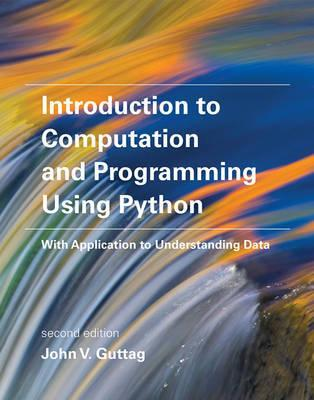
\includegraphics[width=0.8\textwidth]{figs/common/intro-python-book.jpg}
            \end{figure}
        \end{column}
        \begin{column}{0.5\textwidth}
            \begin{tabular}{c|c}
                {\bfseries\blue Actividad} & {\bfseries\blue Punteo} \\
                \midrule
                Tareas y ejercicios & 50\% \\
                Proyecto 0 & 25\% \\
                Proyecto 1 & 25\% \\
                \bottomrule
            \end{tabular}
        \end{column}
    \end{columns}
\end{frame}

\begin{frame}{Recomendaciones}
    \begin{itemize}
        \item Se debe buscar aprender la {\bfseries\blue lógica de programación} y no las recetas vistas en clase.
        \begin{itemize}
            \item Lo importante es aprender a escribir programas para resolver problemas. 
            \item Esto te permite aprender a programar en otro lenguaje más rápidamente.
        \end{itemize}
        
        \item ¿Eres totalmente nuevo en programación? 
            \begin{itemize}
                \item {\bfseries\orange PRACTICA, PRACTICA y ¡PRACTICA!}
                
                \item No temas en probar instrucciones de Python, ¡la computadora no va a explotar!
                
                \item {\bfseries\blue ¡TEN PACIENCIA!}
            \end{itemize}
            
        \item Puedes consultar un sinfín de cursos, blogs, tutoriales y documentación en Internet.
    \end{itemize}
\end{frame}

\begin{frame}{Agenda}
    \begin{itemize}
        \item Introducción a la computación.
        \item Introducción a Python.
    \end{itemize}
\end{frame}

\begin{frame}{¿Qué hace una computadora?}
    \begin{itemize}
        \item Fundamentalmente: 
            \begin{itemize}
                \item Realiza cálculos (hasta billones por segundo).
                \item Guarda los resultados (cientos de GBs).
            \end{itemize}
        \item ¿Qué tipo de cálculos?
            \begin{itemize}
                \item Muy simples: operaciones aritméticas y lógicas.
                \item Los que el programador {\bfseries\blue define}.
            \end{itemize}
    \end{itemize}
\end{frame}

\begin{frame}{Tipos de conocimiento}
    \begin{itemize}
        \item {\bfseries\orange Declarativo}: afirmación o enunciado a partir de un hecho.
            \begin{blurb}
            La raíz cuadrada de $x$ es un número $y$ tal que $y\times y = x$.
            \end{blurb}
        
        \item {\bfseries\orange Imperativo}: una {\blue receta} de cómo hacerlo.
        \begin{blurb}
            \begin{itemize}
                \item Empiece con una deducción $g$. 
                \item Si $g\times g$ está cerca de $x$, deténgase y $g$ es la respuesta.
                \item De lo contrario, su nueva deducción es el promedio de $g$ y $x/g$.
                \item {\blue Repita} el proceso hasta estar cerca de $x$.
            \end{itemize}
            \end{blurb}
    \end{itemize}
\end{frame}

\begin{frame}{Algoritmos}
    \begin{itemize}
        \item Secuencias de {\blue pasos simples} (\textit{atómicos}).
        \item Hay un {\blue flujo de control} que especifica cuándo se ejecuta cada paso.
        \item Existe una forma de determinar {\blue cuando parar}.
    \end{itemize}
    
    \bottomline{Estos ingredientes conforman un algoritmo.}
\end{frame}

\begin{frame}{Tipos de computadoras}
    \begin{itemize}
        \item ¿Qué exactamente es una computadora?
        \item Las computadoras son {\blue máquinas} que capturan la receta.
        \item de programas {\blue fijos} (e.g. calculadora). 
        \item de programas {\blue almacenados}: guardan y ejecutan instrucciones almacenadas en memoria.
    \end{itemize}
\end{frame}

\begin{frame}{Arquitectura básica}
    \centering
    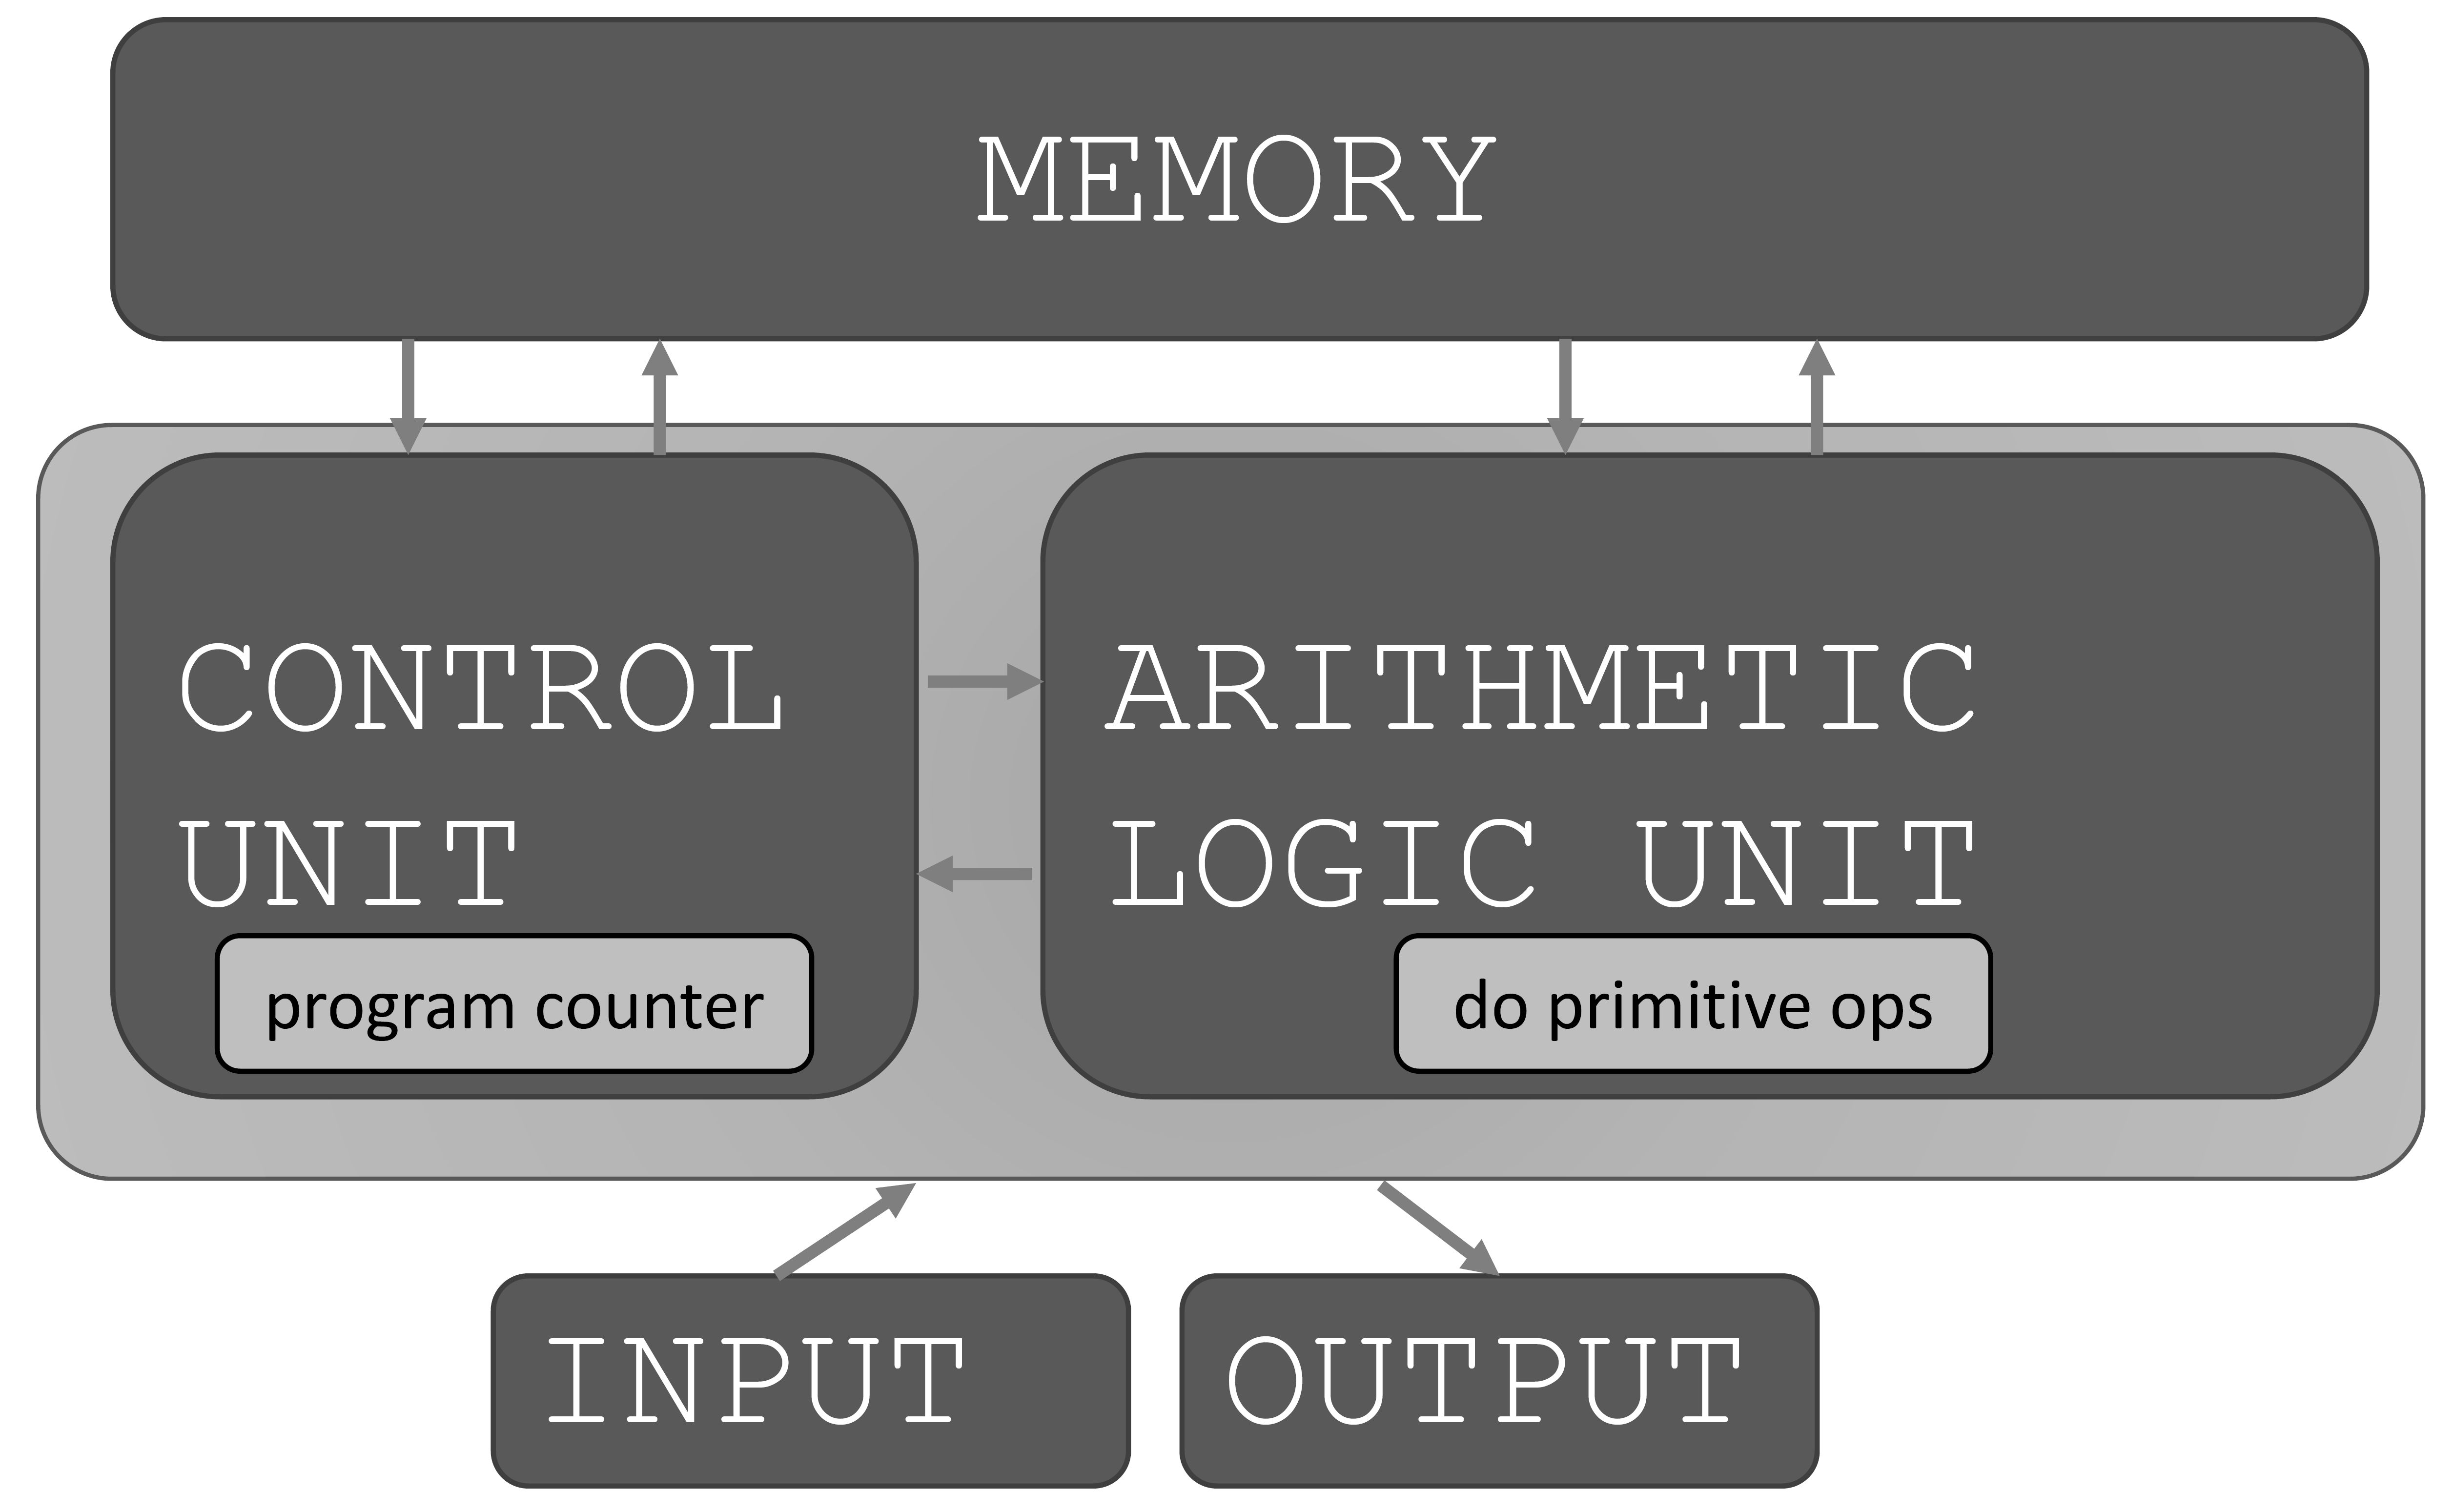
\includegraphics[width=0.9\textwidth]{figs/intro/computer-architecture.png}
\end{frame}

\begin{frame}{Programas almacenados}
    \begin{itemize}
        \item Consisten en una {\orange secuencia de instrucciones} almacenadas en la computadora. 
        \item Construidas a partir de instrucciones {\blue primitivas}:     \begin{itemize}
            \item Aritméticas y lógicas.
            \item Condiciones simples.
            \item Operaciones de memoria.
        \end{itemize}
        
        \item El {\bfseries\blue intérprete} se encarga de ejecutar las instrucciones en orden.
            \item Utiliza pruebas para cambiar el flujo de control en la secuencia.
            \item Se detiene cuando termina la ejecución.
    \end{itemize}
\end{frame}

\begin{frame}{Máquina universal de Turing}
    \begin{cpage}
    ``(...) In 1936, the British mathematician Alan Turing described a hypothetical computing device that has come to be called a {\blue Universal Turing Machine}. The machine had an unbounded memory in the form of 'tape' on which one could write zeroes and ones, and some very simple primitive instructions for moving, reading, and writing to the tape. The {\blue Church-Turing thesis} states that if a function is computable, a Turing Machine can be programmed to compute it.''
    \end{cpage}
\end{frame}

\begin{frame}{Máquina universal de Turing}
    \begin{cpage}
    ``(...) The Church-Turing thesis leads directly to the notion of {\blue Turing completeness}. A programming language is said to be Turing complete if it can be used to simulate a universal Turing Machine. All modern programming languages are Turing complete. As a consequence, anything that can be programmed in one programming language (e.g., Python) can be programmed in any other programming language (e.g., Java). Of course, some things may be easier to program in a particular language, but all languages are fundamentally equal with respect to computational power.''
    \end{cpage}
\end{frame}

\begin{frame}{Primitivas básicas}
    \begin{itemize}
        \item Turing mostró que se puede computar {\bfseries\blue cualquier cosa} con algunas primitivas básicas.
        \item Los lenguajes de programación modernos tienen primitivas más convenientes.
            \begin{itemize}
                \item Análogamente a un lenguaje natural, tienen palabras, sintaxis, semántica y significado.
            \end{itemize}
            
        \bottomline{Cualquier tarea computable en un lenguaje, es computable en cualquier otro lenguaje de programación.}
    \end{itemize}
\end{frame}

\begin{frame}{Construyendo expresiones}
    \begin{itemize}
        \item Las {\blue expresiones} son combinaciones (complejas) legales de primitivas en un lenguaje de programación (LP). 
        \item Las expresiones y cómputos tienen valores y significados en el lenguaje. 
        \item Construcciones primitivas: 
            \begin{itemize}
                \item Español: palabras.
                \item LP: números, cadenas de texto, operadores.
            \end{itemize}
    \end{itemize}
\end{frame}

\begin{frame}{Sintaxis}
    \begin{itemize}
        \item Se refiere a las reglas que especifican {\blue secuencias correctas} de símbolos que pueden ser usadas para formar expresiones en el lenguaje.
        
        \item Por ejemplo: ``Niño gato perro'' no es sintácticamente válida en español.
        \item En Python, una secuencia correcta es \lstinline|1.5+1.6|, pero no \lstinline|1.5 1.6|.
    \end{itemize}
\end{frame}

\begin{frame}{Semántica estática}
    \begin{itemize}
        \item Se refiere a que las cadenas sintácticamente válidas tengan significado. 
        
        \item ``Yo estamos hambriento'' no es semánticamente válida.
        
        \item En Python: 
        \begin{itemize}
            \item \lstinline|3.2*5| es válida.
            \item \lstinline|3+"hola"| no es válida.
        \end{itemize}
    \end{itemize}
\end{frame}

\begin{frame}{Semántica}
    \begin{itemize}
        \item Se refiere al significado asociado a las cadenas {\blue sintácticamente válidas} y sin errores {\blue semánticos estáticos}.
        
        \item ``Estudiar el PES es alegre'' puede tener diversos significados.
        
        \item Los lenguajes de programación están diseñados para tener solo un significado. 
            \begin{itemize}
                \item Aunque en ocasiones, este puede no ser el deseado por el programador.
            \end{itemize}
    \end{itemize}
\end{frame}

\begin{frame}{Tipos de errores}
    \begin{itemize}
        \item {\bfseries\orange de sintaxis}: 
            \begin{itemize}
                \item {\blue Muy} comunes y fácilmente detectables.
            \end{itemize}
        
        \item {\bfseries\orange de semántica estática}:
            \begin{itemize}
                \item Algunos programan revisan antes de permitir la ejecución.
                \item Pueden causar comportamiento impredecible.
            \end{itemize}
            
        \item Sin errores semánticos pero {\bfseries\orange diferente significado al deseado}: 
            \begin{itemize}
                \item Los programas se detienen, fallan o se ejecutan para siempre.
                \item La respuesta puede no ser la esperada.
            \end{itemize}
    \end{itemize}
    
    \bottomline{Los programas deben escribirse de tal forma que, si fallan, el hecho de que no funcionen sea evidente.}
\end{frame}

% Introducción a Python

\begin{frame}{¿Python?}
    \begin{columns}
        \begin{column}{0.4\textwidth}
            \begin{figure}
                \centering
                %\includesvg[width=\textwidth]{figs/common/python-powered-h}
                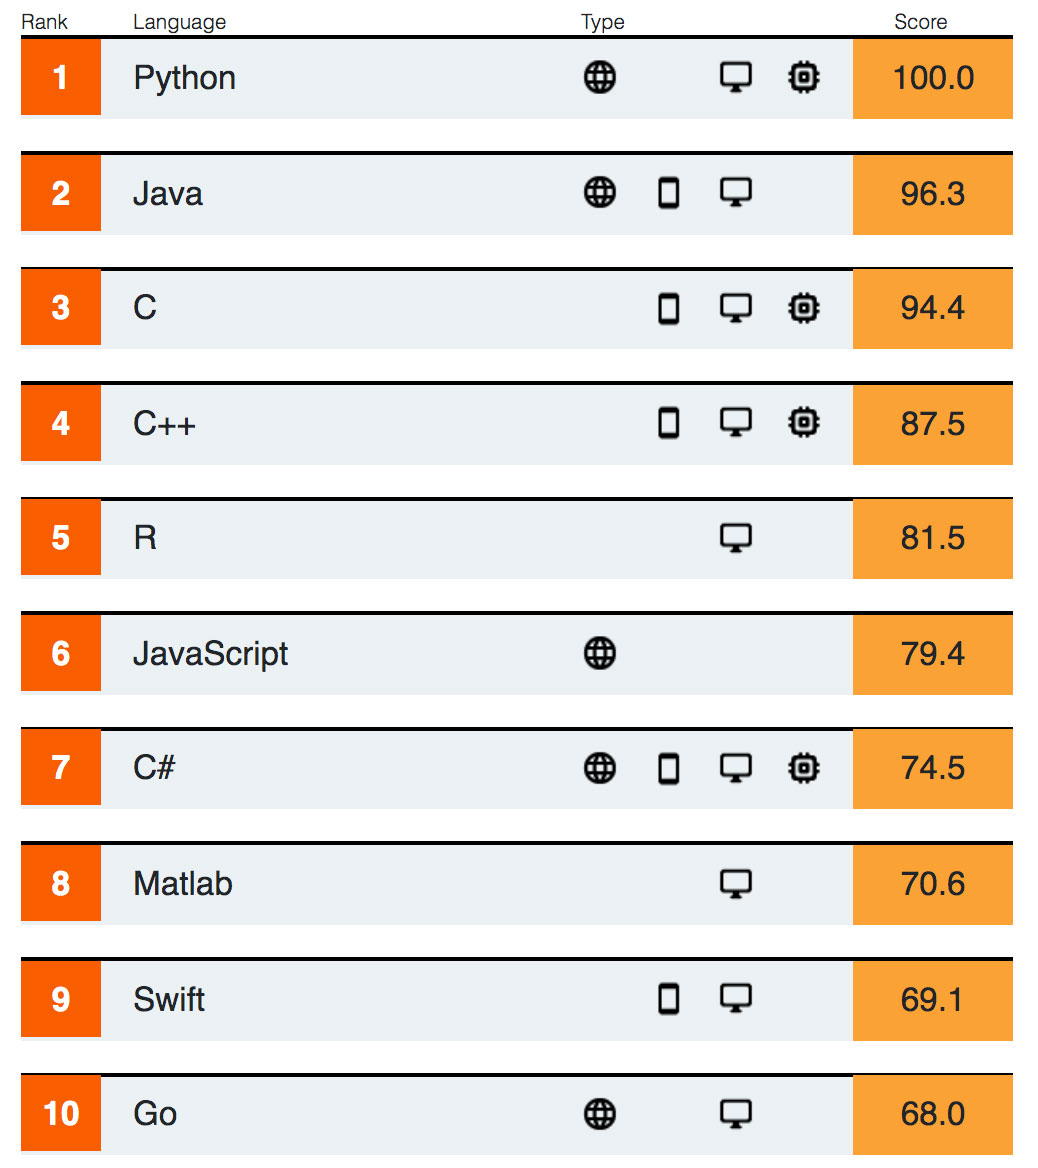
\includegraphics[width=0.9\textwidth]{figs/common/python-ranking.jpg}
            \end{figure}
        \end{column}
        \begin{column}{0.6\textwidth}
            \begin{itemize}
                \item Es un lenguaje {\blue interpretado} de código abierto, relativamente {\bfseries\orange simple}, y excelente opción para {\blue principiantes}.
                \item Es de propósito general:
                    \begin{itemize}
                        \item Aplicaciones de escritorio y web.
                        \item Interacción con \textit{hardware}, videojuegos.
                        \item Computación científica (\textit{data science}, AI).
                    \end{itemize}
                \item Utilizado en la industria, academia y por muchos profesionales: 
                    \begin{itemize}
                        \item Google, Amazon, Dropbox, Instagram, Mr. Robot.
                    \end{itemize}
            \end{itemize}
        \end{column}
    \end{columns}
\end{frame}

\begin{frame}{Python es interpretado}
    \begin{itemize}
        \item Los lenguajes {\blue compilados} convierten el código fuente a código de máquina. 
        \item En los lenguajes {\blue interpretados}, el intérprete convierte la fuente a su estructura interna y ejecuta línea por línea.
    \end{itemize}
    \begin{figure}
        \centering
        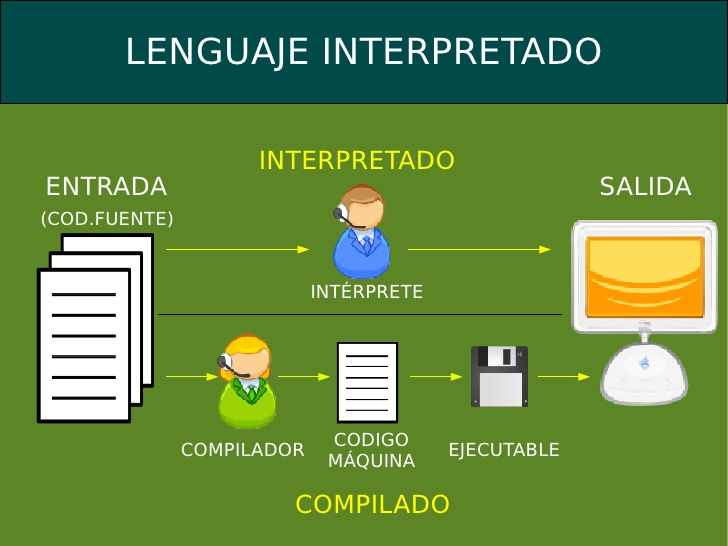
\includegraphics[width=0.6\textwidth]{figs/intro/python-interpretado.jpg}
    \end{figure}
\end{frame}

\begin{frame}{Programas de Python}
    \begin{itemize}
        \item Un programa es una secuencia de {\blue definiciones} e {\blue instrucciones}.
            \begin{itemize}
                \item Las definiciones son {\orange evaluadas}: \lstinline|a=2|, \lstinline|x,y = y,x|.
                \item Las instrucciones son {\orange ejecutadas} por el intérprete: \lstinline|print("Hola amigo")|.
            \end{itemize}
            
        \item Las instrucciones indican al intérprete {\blue qué hacer}.
        
        \item Pueden ser dadas directamente en la {\blue línea de comandos} o en un {\blue archivo} de texto.
            \begin{itemize}
                \item Jupyter notebooks.
            \end{itemize}
    \end{itemize}
\end{frame}

\begin{frame}{Objetos}
    \begin{itemize}
        \item Los programas de Python manipulan {\bfseries\blue objetos}.
        
        \item Cada objeto tiene un tipo asociado, que define lo que se puede hacer con él.
        
        \item Los objetos pueden ser de tipo: 
        \begin{itemize}
            \item {\bfseries\orange escalar}: indivisibles (atómicos). 
            \item {\bfseries\orange no escalares}: poseen estructura interna.
        \end{itemize}
    \end{itemize}
\end{frame}

\begin{frame}{Objetos escalares}
    En Python, existen 4 tipos de objetos escalares
    \begin{itemize}
        \item \lstinline|int| --- representa número enteros: \lstinline|2|, \lstinline|3-2|. 
        \item \lstinline|float| --- representa números reales: \lstinline|3.14159|
        \item \lstinline|bool| --- representa valores booleanos: \lstinline|True| y \lstinline|False|\footnote{Python es \textit{case sensitive}.}.
        \item \lstinline|NoneType| --- toma el valor especial \lstinline|None|.
    \end{itemize}
    
    \begin{itemize}
        \item Conversión de tipos con las funciones \lstinline|int()|, \lstinline|float()|, \lstinline|bool()|.
    \end{itemize}
    
    \bottomline{Podemos utilizar la función \lstinline|type()| para ver el tipo de un objeto.}
\end{frame}

\begin{frame}[fragile]{Impresión en consola}
    \begin{itemize}
        \item Para mostrar salida de un código al usuario, utilizamos el comando \lstinline|print|. {\blue Utilizado en archivos de código o \textit{scripts}}.
        
        \begin{blurb}
        \centering 
        \lstinline|print("Hola amigos")|
        \end{blurb}
        
        \item Cuando {\blue estamos en la consola}, basta con escribir el nombre de la variable o expresión para mostrar un resultado. 
        
\begin{lstlisting}
a=2
b=3
# Imprimir el resultado
a+b
5
\end{lstlisting}
        
    \end{itemize}
\end{frame}

\begin{frame}{Expresiones}
    \begin{itemize}
        \item Se {\bfseries\orange combinan objetos y operadores} para formar expresiones.
        
        \item Una expresión tiene un {\bfseries\orange valor}, el cual tiene un tipo. 
        
        \item Sintaxis: \lstinline|<objeto> <operador> <objeto>|
    \end{itemize}
\end{frame}

\begin{frame}{Operadores}
    \begin{itemize}
        \item Aritméticos: \lstinline|+ - * / // \% **|
        \item Comparación: \lstinline|== < > <= >=|
        \item Lógicos: \lstinline|and|, \lstinline|or| y \lstinline|not|
        \item Asignación (une nombre a valor): \lstinline|=|
    \end{itemize}
    \bottomline{Notar la diferencia entre \lstinline|=| y \lstinline|==|.}
    
    Considerar la precedencia de los operadores:
    \begin{itemize}
        \item Paréntesis
        \item \lstinline|**|
        \item \lstinline|*|
        \item \lstinline|/|
        \item \lstinline|+| y \lstinline|-|
    \end{itemize}
    
    \bottomline{Ejecutados de izquierda a derecha, en orden de aparición.}
\end{frame}

\begin{frame}[fragile]{Expresiones más abstractas}
    \begin{itemize}
        \item Nombres de variables $\Rightarrow$ {\bfseries\blue reutilizar} nombres y valores.
\begin{lstlisting}
pi = 3.14159
radius = 2.2
area = pi*(radius**2)
\end{lstlisting}

        \item Se vale referir a la misma variable: 
\begin{lstlisting}
radius = radius + 1
\end{lstlisting}

        \item El valor de \lstinline|area| no cambia hasta computarla nuevamente.
    \end{itemize}
\end{frame}

%-----------------------------------------------------------------
% Termina el contenido de la presentación
%-----------------------------------------------------------------
\end{document}